\documentclass[10pt,letterpaper]{article}
\usepackage[T1]{fontenc}
\usepackage{lmodern}
\usepackage[margin=0.78in]{geometry}
\usepackage{amsmath,amssymb,booktabs,array,graphicx,longtable,fancyhdr}
\usepackage[hidelinks]{hyperref}
\usepackage{listings}
\makeatletter\let\tableinput\@@input\makeatother
\newcommand{\degC}{\ensuremath{^{\circ}\mathrm{C}}}
\newcommand{\us}{\ensuremath{\mu\mathrm{s}}}
\newcommand{\snap}{https://github.com/KuznetsovKarazin/lut-kan-native/tree/db39238c1467169b65ff1f3581945e57ee7ffd7a}
\hypersetup{pdftitle={Supplement: Accuracy, Storage, and Update Cost in Reference-Assisted Sensor Calibration},pdfauthor={Oleksandr Kuznetsov}}
\renewcommand{\thetable}{S\arabic{table}}
\pagestyle{fancy}\fancyhf{}\lhead{Embedded sensor calibration: supplementary material}\rhead{8 November 2026}\cfoot{\thepage}
\setlength{\headheight}{13pt}
\setlength{\parindent}{0pt}\setlength{\parskip}{5pt}
\lstset{basicstyle=\ttfamily\footnotesize,breaklines=true,columns=fullflexible,keepspaces=true,frame=single,rulecolor=\color{black},showstringspaces=false}
\usepackage{xcolor}
\begin{document}
\begin{center}
{\Large\bfseries Supplementary Material}\par
\vspace{4pt}{\large Accuracy, Storage, and Update Cost in Reference-Assisted Sensor Calibration}\par
\vspace{5pt}Oleksandr Kuznetsov\par
Working revision, 8 November 2026; evidence: \texttt{db39238} and \texttt{0b828da}
\end{center}

\section*{S1. Scope and interpretation}
This supplement provides all static and sequential mean-error comparisons, paired intervals, measured update times, memory accounting, and reproduction instructions. Accuracy and drift are synthetic; physical boards establish execution time and numerical agreement.

In the original study, each scenario and budget has eight virtual units with three repetitions each. Repetitions are averaged within units before aggregation or resampling. Tables S1--S5 use degrees Celsius for both NTC cases and $\log_{10}(\mathrm{lux})$ for LDR; these units must not be pooled. Source JSON retains full precision, per-unit statistics, RMSE, and additional diagnostics.

\section*{S2. Complete static comparison}
Table S1 includes all seven equal-capacity methods. ``mLUT'' uses decreasing-constrained initial fitting. ``KAN'' denotes a scalar spline-plus-SiLU edge. Table S2 reports smaller-payload fitted Steinhart--Hart/log-linear physical models and selected polynomials separately.

\begin{table}[!ht]
\centering\caption{Mean noisy-grid MAE for all equal-capacity static models.}
\small\setlength{\tabcolsep}{4pt}
\begin{tabular}{lrrrrrrrrr}\toprule
Scenario & $B$ & Bytes & LUT f32 & LUT i16 & mLUT f32 & mLUT i16 & Cubic & Horner & KAN\\\midrule
\tableinput tables/all_static.tex
\bottomrule\end{tabular}
\end{table}

\begin{table}[!ht]
\centering\caption{Smaller-payload physical and polynomial references.}
\small\begin{tabular}{lrrr}\toprule
Scenario & $B$ & Physical model & Selected polynomial\\\midrule
\tableinput tables/small_references.tex
\bottomrule\end{tabular}
\end{table}

\clearpage
\section*{S3. Complete sequential comparison}
Tables S3 and S4 jointly cover all nine sequential methods. Each cell averages the final 401-point grid MAE after 384 new labelled references over eight units and three repetitions. The two budgets count the initial references; the additional 384 references are not free calibration data. Projected variants use decreasing coefficient projection after each update, including initialization. The frozen methods receive the same stream but do not update from its labels.

\begin{table}[!ht]
\centering\caption{Final MAE: frozen, projected NLMS, and RLS comparisons.}
\footnotesize\setlength{\tabcolsep}{4.5pt}
\begin{tabular}{lrlrrrrrr}\toprule
&&&\multicolumn{2}{c}{Frozen}&\multicolumn{2}{c}{Projected NLMS}&\multicolumn{2}{c}{RLS}\\
Scenario & $B$ & Drift & LUT & Cubic & LUT & Cubic & Cubic & Polynomial\\\midrule
\tableinput tables/all_online.tex
\bottomrule\end{tabular}
\end{table}

\begin{table}[!ht]
\centering\caption{Final MAE of the remaining three methods.}
\footnotesize\begin{tabular}{lrlrrr}\toprule
Scenario & $B$ & Drift & Frozen polynomial & LUT NLMS & Cubic NLMS\\\midrule
\tableinput tables/other_online.tex
\bottomrule\end{tabular}
\end{table}

The development seed is 2026110800 and the confirmation seed is 2026110801. Development uses four virtual units, two repetitions, all three scenarios, both initial reference budgets, and all drift modes. Global NLMS rates are selected from $\{0.05,0.2,0.5,1\}$ and RLS forgetting factors from $\{0.98,0.995,1\}$. The selected values are 0.5 and 0.98, respectively. Development comprises 3168 candidate trajectories; independent confirmation comprises 3888 trajectories. No confirmation trajectories failed numerically, and no projected coefficient-order violations were recorded.

\clearpage
\section*{S4. Paired comparison and numerical diagnostics}
The static endpoint below is the paired difference between float32 LUT MAE and compiled Horner MAE. Negative values favor the LUT. Each bootstrap draw samples eight units with replacement, retaining the within-unit pairing and averaging the three repetitions first. Intervals are 95\% percentile intervals from 2000 draws. They are exploratory and have no multiplicity adjustment. They describe variation in the stated synthetic experiment, not uncertainty across physical manufactured sensors.

\begin{table}[!ht]
\centering\caption{Paired mean MAE difference: LUT float32 minus Horner.}
\small\begin{tabular}{lrrrr}\toprule
Scenario & $B$ & Bytes & Mean difference & 95\% interval\\\midrule
\tableinput tables/paired.tex
\bottomrule\end{tabular}
\end{table}

The source spline underlying each Horner model is $C^2$ before coefficient rounding. The maximum recorded normalized value jump after float32 conversion is $1.79\times10^{-7}$, and the maximum normalized first-derivative jump is $8.72\times10^{-7}$. These are representation-conversion diagnostics, not sensor error estimates. Dense-grid, exact-knot, adjacent-float, and clipped-endpoint tests compare the compiled polynomial with independent spline evaluation.

The fixed MCU numerical gate is $0.002\,\degC$. Maximum prediction, scaled checkpoint-state, and timed final-state discrepancies are $0.00001526$, $0.00001490$, and $0.00001192\,\degC$, respectively. Each capture retains four static accuracy records, 50 inference/overhead timings, 96 state checks, 12 online accuracy records, 120 update timings, and 30 update-overhead records. Raw and parsed evidence is retained for all four sessions.

Full target-precision trajectory replay confirms that the unprojected MCU fixture remains decreasing for all 384 updates in each schedule. Projected and ordinary trajectories coincide, and PAVA performs no block merges. No inference about active-projection accuracy benefits or worst-case PAVA timing is made. Full replay of the original 432 streams found zero changed LUT initial states or updates. Cubic projection changed 42 initial states and 557 updates in 42 trajectories. Affected groups and physical-unit correction sizes are retained in the revision audit. The target fixture is not a comprehensive projection workload.

\section*{S5. Protocol details needed for reproduction}
The initial quantity grid covers the declared operating range; interior references receive a uniform jitter bounded by one quarter of the nominal spacing. Validation uses interior indices 2, 5, 8, and so on, with all validation labels counted in $B$. All models are refitted on the complete initial reference set after selecting their settings. Regularization is selected after the actual coefficient encoding or Horner conversion.

The independent test quantities are the 401 interior points of a 403-point uniform grid. Test ADC noise uses an independent random generator. Online reference blocks cover 32 equal quantity bins, in independently shuffled order. Checkpoints are $0,32,64,96,127,128,129,132,144,160,192,224,256,320,384$. Updates cannot access evaluator truth or future labels; transforms remain fixed.

\clearpage
\section*{S6. All measured update times and implementation sizes}
Times in Table S6 are gross microseconds per labelled update, aggregated as the median of two session medians. Each session times ten complete 384-reference trajectories. States are reset outside the timed region. MAE is evaluated using the target fixture's final independent noisy grid; it is not the aggregate error in Table S3. Board-to-board reported errors agree to approximately $10^{-7}\,\degC$; the C3 values are tabulated.

\begin{table}[!ht]
\centering\caption{Full update time and final synthetic error for every drift schedule.}
\small\begin{tabular}{llrrr}\toprule
Drift & Method & Mega (\us{}) & C3 (\us{}) & MAE (\degC)\\\midrule
\tableinput tables/all_hardware_updates.tex
\bottomrule\end{tabular}
\end{table}

The gross static overhead medians are 12.3~\us{} on Mega2560 and 0.700~\us{} on ESP32-C3. They are recorded separately and not subtracted from the primary results. Both boards use two warm, command-driven sessions after a single upload. There is one board per architecture. Repeating the same fixture provides timing repeatability information; it does not supply independent sensor samples or a worst-case execution-time bound.

\begin{table}[!ht]
\centering\caption{Separate deployment builds: absolute Flash and static RAM, in bytes.}
\small\begin{tabular}{lrrrr}\toprule
&\multicolumn{2}{c}{Mega2560}&\multicolumn{2}{c}{ESP32-C3}\\
Implementation & Flash & Static RAM & Flash & Static RAM\\\midrule
Empty harness&734&21&218848&13484\\
LUT32 float32&2340&165&219276&13484\\
LUT60 int16&2404&165&219382&13484\\
Compact cubic32&2842&165&219718&13484\\
Horner8&2324&165&219296&13484\\
LUT NLMS&2834&169&219586&13636\\
LUT projected NLMS&3376&329&219964&13796\\
Cubic NLMS&3424&169&220074&13636\\
Cubic projected NLMS&3962&329&220460&13796\\\bottomrule
\end{tabular}
\end{table}

These absolute build sizes include framework/startup code and compiler alignment. They are distinct from model payload and from the larger acquisition firmware containing reference data, all models, and serial validation. Inference payload is 144 bytes for all four models. NLMS persistent state is 148 bytes; PAVA adds 160 bytes of reusable caller workspace. Local basis scratch and call stack are extra. AVR initialization snapshots are placed in Flash and copied before timing. Neither static RAM nor a compiler stack estimate is a measured peak-stack value.

The build environment uses PlatformIO atmelavr 5.1.0 with AVR GCC 7.3.0 and Arduino AVR 5.2.0, and espressif32 6.12.0 with GCC 8.4.0 and Arduino ESP32 3.20017.241212. Target builds disable fast-math and floating-point contraction. Twenty build configurations completed; AVR program-memory fixture addresses were checked against the near-Flash access limit. The committed build reports and configuration files are authoritative for exact flags and package versions.

\clearpage
\section*{S7. Code, evidence, and reproduction}
The original tables above remain unchanged in scope. New revision analyses follow in S8--S12. The public repository is \url{https://github.com/KuznetsovKarazin/lut-kan-native}. This manuscript uses experimental snapshot
\begin{center}\texttt{db39238c1467169b65ff1f3581945e57ee7ffd7a}.\end{center}
The research branch may advance; use the immutable snapshot for the reported evidence. Relevant links are:
\begin{itemize}
\item \href{\snap/experiments/sensor_recovery}{Experiment source, protocols, and result directories}.
\item \href{\snap/experiments/sensor_recovery/results/matched_adaptation_20261108}{Static and sequential summaries, per-unit values, paired intervals, and checkpoint curves}.
\item \href{\snap/experiments/sensor_recovery/results/matched_boards_20261108}{Matched-board comparison and measurement scope}.
\item \href{\snap/experiments/sensor_recovery/results/c3_matched_20261108}{ESP32-C3 raw captures and audit}, and \href{\snap/experiments/sensor_recovery/results/mega_matched_20261108}{Mega2560 raw captures and audit}.
\item \href{\snap/experiments/sensor_recovery/results/matched_mcu_20261108}{Numerical preparation and separate-build records}. Historical reports in this directory describe the preparation checkpoint; the subsequent board captures supply the real timings used here.
\end{itemize}

\textbf{Rebuilding the paper.} The portable manuscript archive contains \texttt{main.tex}, \texttt{supplement.tex}, \texttt{references.tex}, \texttt{IEEEtran.cls}, all vector figures, editable SVG/PNG exports, table fragments, exact JSON figure inputs, and the generation script. No hardware or raw-trajectory download is required to rebuild its figures and tables. The code first reads the repository results when available; otherwise it reads the included input snapshot. From the manuscript directory:
\begin{lstlisting}
python make_assets.py
latexmk -pdf main.tex
latexmk -pdf supplement.tex
\end{lstlisting}
Figure generation uses Python with NumPy and Matplotlib. The verified environment uses Python 3.12.14, NumPy 2.3.5, and Matplotlib 3.10.8. The experiment additionally uses SciPy 1.17.0. Input SHA-256 values are in \texttt{data/source\_hashes.json}. Figure regeneration does not rerun or alter the experiments.

\textbf{Regenerating the synthetic campaign.} Use a fresh output directory. From the repository root, the following commands reproduce the declared stages with the script's frozen defaults:
\begin{lstlisting}
git checkout db39238c1467169b65ff1f3581945e57ee7ffd7a
export OPENBLAS_NUM_THREADS=1
export OMP_NUM_THREADS=1
python experiments/sensor_recovery/run_matched_adaptation.py static --out reproduced/static
python experiments/sensor_recovery/run_matched_adaptation.py development --out reproduced/development
python experiments/sensor_recovery/run_matched_adaptation.py confirmation --out reproduced/confirmation --selection reproduced/development/selected_parameters.json
python experiments/sensor_recovery/report_matched_adaptation.py reproduced
\end{lstlisting}
The \texttt{run\_info.json} files retain exact commands, seeds, source hashes, software versions, and output hashes from the original runs. The local protocol-freeze and later public-commit mapping are documented in \path{publication_provenance.json}; public commit dates must not be interpreted as preregistration dates.

\textbf{Raw-data availability boundary.} The public Git tree contains the source, numerical summaries and per-unit aggregates, manuscript inputs, and raw MCU logs. The complete synthetic reference streams and trajectory states reside in the separately preserved archive \path{IEEE_Sensors_Matched_Adaptation_Data_2026-11-08.zip} (140570539 bytes). That large archive is not hosted in the Git tree. Its manifest lists six deterministic compressed JSONL files and SHA-256 values. The archive SHA-256 is:
\begin{center}\scriptsize\texttt{c1594e1668d1c0c0f1bcd4e1c27ac91bfec2393a182fd468e37483e02ac6e1f3}.\end{center}
The commands above regenerate the synthetic observations and predictions. A separate public data deposit and DOI have not been claimed. The physical-board recordings cannot be recreated by a host simulation; new timings require new hardware captures under the documented acquisition protocol.



\clearpage
\section*{S8. Additional protocol and pseudocode}
The revision protocol was written locally before the new simulations. Seeds are 2026110810 for development and 2026110811 for confirmation. This is additional analysis after review, not retroactive preregistration. Original seeds, evidence and records remain separate. Tests check generator parity, inverse correctness, exclusion of test labels from selection, prefix causality, and endpoint correction. Perturbing all future labels/inputs after sample 128 leaves every earlier new-method checkpoint unchanged.

\textbf{Algorithm 1: fit and select.} Each reference is counted once toward $B$, even when it participates in several internal fits. The input transform uses the complete initial ADC set; output scaling uses the declared range. Neither uses test truth.
\begin{lstlisting}
Input: B initial pairs, fixed family/capacity, candidate grid
Construct fixed transforms and initial basis matrix.
Partition references: original holdout or five interleaved folds.
For each candidate regularizer (or polynomial degree):
    For each validation fold:
        Fit penalized least squares on remaining references.
        Apply declared storage precision/encoding.
        Evaluate squared residuals on this validation fold.
    Average validation residuals; keep the lowest-scoring candidate.
Refit selected candidate using all B initial references.
Store encoded coefficients and transforms; evaluate independent tests.

default ties: first candidate in the frozen ordered grid
CV folds: reference index modulo 5

a noisy independent test set is never a selection fold
\end{lstlisting}

\textbf{Algorithm 2: one NLMS update with optional monotonicity.} The original measured projected implementation invokes full PAVA unconditionally. The guarded path below is an additional tested implementation and has no measured hardware timing. In host experiments the update intermediate is float64, then state is stored as float32; target kernels use float32 throughout.
\begin{lstlisting}
Input: fixed transforms, coefficients c, new (ADC, reference), eta
Normalize the new pair; compute the 2 or 4 active basis weights b.
Predict p = dot(b, c); residual e = reference_normalized - p.
v = c + eta * e * b / (dot(b, b) + 1e-6).
If decreasing coefficients are required:
    If any adjacent pair violates v[j] >= v[j+1]:
        Initialize one block per coefficient, weight 1.
        Scan blocks left to right.
        While previous block mean < current block mean:
            Merge the two blocks using their weighted mean.
            Recheck against the preceding block.
        Expand block means back into coefficient vector v.
Store v as float32. Return the pre-update prediction if required.
\end{lstlisting}
Projection is Euclidean on coefficient values, not on sampled function errors. Decreasing coefficients are sufficient for monotone output in these bases. Initial constrained LUT fitting in the original static study solves the constrained objective; this differs from projecting a completed unconstrained fit.

\textbf{Causal reference baselines.} Two-point correction retains the lowest and highest \emph{frozen-model predictions} and their noisy labels within each completed block of 32. It estimates gain and offset from those pairs, then applies that correction until the next block completes. It does not use true quantities to choose endpoints. All-history and recent-64 batch models include initial references and only the consumed stream prefix; refits occur at the 15 declared checkpoints. Smoothing remains that of the initial model. These schedules and estimator choices are explicit limitations, not optimized representatives of every affine or batch method.

\textbf{Memory.} A two-point implementation needs the frozen model, gain/offset, two candidate input-output pairs and a counter; alignment and arithmetic can change the final size. Decaying NLMS additionally needs its schedule parameter and sample counter. Batch buffers alone require $8(B+t)$ bytes or $8\times64=512$ bytes when pairs are float32. Factorization/design-matrix workspace is additional. These new algorithms were evaluated on the host; no MCU state size or latency is inferred from host execution.

\clearpage
\section*{S9. Cross-validation and sensitivity results}
Table S8 reports all nominal equal-capacity selection comparisons. There are eight units and two repetitions per cell, from the new confirmation seed. Both selectors refit on the same full set of initial references. The full JSON also supplies ideal MAE, noisy MAE, maximum observed errors, per-unit values, and the exact-generator inverse benchmark. Large errors from held-out selection are retained rather than clipped out of summaries.
\begin{table}[!ht]
\centering\caption{New nominal noisy MAE: holdout versus fivefold cross-validation.}
\small\begin{tabular}{lrrrrrr}\toprule
&&&\multicolumn{2}{c}{Float32 LUT}&\multicolumn{2}{c}{Compact cubic}\\
Scenario & $B$ & Bytes & Holdout & CV & Holdout & CV\\\midrule
\tableinput tables/cv_all.tex
\bottomrule\end{tabular}
\end{table}

The one-factor-at-a-time study keeps initial label noise and averaging unchanged. Noise levels 0.25 and 4 LSB refer to each individual conversion, before 16-sample averaging. Tolerance factors multiply half-widths about the nominal $R_0$, $\beta$ or $\gamma$, not the parameter means. Distortion amplitude is in ADC LSB; frequency counts cycles over normalized divider output, not over temperature. All evaluated distorted transfer functions are monotone over the declared temperature range, so bisection supplies their oracle inverse. Hidden generator parameters are used only for this evaluator, never for fitting any baseline.

These controls improve interpretation but do not make the generator a physical population model. The revised main text treats the original bootstrap intervals as descriptive. Repetitions and virtual units do not become independent physical instruments merely because their random seeds differ. No multiplicity-adjusted superiority claim is made.

\section*{S10. New sequential baselines and parameter selection}
The original nine methods are rerun on the new confirmation streams. Ten additional method configurations yield 19 trajectories per stream: two decaying NLMS, two extended-grid RLS, two two-point corrections and four batch refits. Development selects $\tau=512$ for both decaying methods, cubic RLS forgetting 0.98 and polynomial RLS forgetting 0.95. Every candidate and every run is retained. There were zero numerical failures in 2304 development and 5472 confirmation trajectories.

For the development integrated normalized-MSE objective, cubic RLS scores at forgetting factors 0.90, 0.95, 0.98, 0.995, and 1 are $2.67\times10^{-4}$, $1.38\times10^{-5}$, $9.37\times10^{-6}$, $1.87\times10^{-5}$, and $2.70\times10^{-5}$. Polynomial scores are $5.80\times10^{-6}$, $5.60\times10^{-6}$, $8.50\times10^{-6}$, $1.84\times10^{-5}$, and $2.67\times10^{-5}$. The expanded grid therefore has interior selected values. No claim of a continuous optimum follows from that grid.

\clearpage
\begin{table}[!ht]
\centering\caption{Revision final MAE: cubic baselines and extended-grid RLS.}
\scriptsize\setlength{\tabcolsep}{3pt}
\begin{tabular}{lrlrrrrrrrr}\toprule
&&&\multicolumn{6}{c}{Cubic family}&\multicolumn{2}{c}{RLS, extended grid}\\
Scenario & $B$ & Drift & Frozen & NLMS & Decay & 2-point & Batch all & Batch 64 & Cubic & Poly.\\\midrule
\tableinput tables/revision_online.tex
\bottomrule\end{tabular}
\end{table}

The machine-readable \path{data/revision_summary.json} contains the complete 19-method table, including LUT variants and both RLS configurations, with final and checkpoint-integrated MAE. \path{data/revision_curves.json} contains every mean checkpoint. All error units follow the scenario, and cannot be averaged across temperature and logarithmic illuminance. The paired input streams and method states are in the separately preserved revision raw-data archive; commands below regenerate them.

\textbf{Projection audit.} Both projected families were replayed on all 432 original streams. This checks 331776 actual update events, not just equality of rounded endpoint means. LUT: zero changed initial states and zero changed updates. Cubic: 42 changed initial states and 557 changed updates across 42 streams. Thus PAVA is inactive for LUT under this generator but not inactive for every cubic trajectory. The audit does not establish a benefit from those cubic corrections. The optional order guard is verified to preserve already-decreasing vectors exactly and to invoke PAVA on an intentionally violated vector; its timing is not substituted for the original measurements.

\section*{S11. Recovered reference timings and restricted decision map}
The earlier optimized-suite pilot has seed 20261108, distinct from the matched suite's 2026110801. Each board has two sessions, each with ten 2048-call batches. Table S10 reparses all four raw logs and aggregates session medians. The stored JSON is reproduced exactly, with raw/result hashes checked against sidecars. The original acquisition archives recorded firmware hashes but did not include firmware images; these are source/serial audits, not device firmware attestation. The existing matched archives have their own stronger image preservation and identity records.

\begin{table}[!ht]
\centering\caption{Earlier pilot: measured references at their actual payloads.}
\small\begin{tabular}{lrrrr}\toprule
Model / payload & Mega (\us{}) & C3 (\us{}) & MAE (\degC) & Maximum (\degC)\\\midrule
\tableinput tables/recovered_hardware.tex
\bottomrule\end{tabular}
\end{table}

The pilot includes a fitted degree-9 Chebyshev polynomial and Steinhart--Hart model. The LUT is fitted with a decreasing constraint; its float32/int16/uint8 variants use the same 32-node source. The spline uses 16 coefficients, or 13 expanded pieces; expansion changes storage from 80 to 224 bytes while preserving the represented function to target rounding. These details differ from matched-payload capacity selection. Neither times nor error values are moved between fixtures.

\clearpage
\begin{figure}[h!]
\centering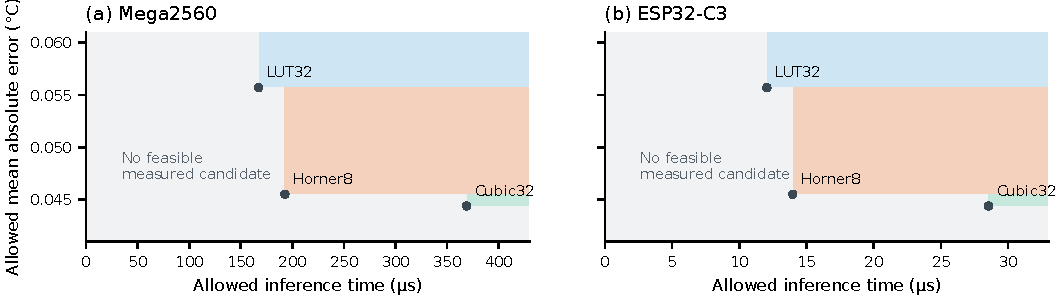
\includegraphics[width=.96\textwidth]{figures/decision_regions.pdf}
\caption{Restricted illustrative decision map from the original matched fixture. It selects only among the four timed 144-byte candidates, at median time and finite-grid MAE. It omits smaller polynomial/physical references and is not a universal deployment rule, accuracy guarantee, or deadline guarantee.}
\end{figure}

\textbf{Prospective matched-reference suite.} A separate prepared suite evaluates the same six static families on the matched fixture, including a 56-byte polynomial and 32-byte physical model. It supports Mega2560 and ESP32-C3, with an optional ESP32-S3-DevKitC-1 UART environment at 240 MHz. It preserves all historical captures. Portable float32 checks give maximum gaps below $5.22\times10^{-5}\,\degC$ for the two new kernels. Compilation and host validation are not additional board measurements. Its purpose is consolidation and optional FPU comparison; the recovered pilot already establishes real execution of the small references.

\section*{S12. Prospective physical validation and reproducibility}
\textbf{A small physical campaign, not executed.} A useful next study would use at least three individual NTC units, the intended divider/ADC/reference-voltage chain, and a traceably calibrated reference thermometer in a stirred bath or stable chamber. Select a safe common temperature range supported by the sensor encapsulation and reference. Fix calibration and held-out setpoints before fitting; acquire both heating and cooling traversals in at least two separate cycles. Record time-resolved ADC values, reference readings, settling criteria, averaging, excitation current, supply/reference voltage and unit identifiers. Repeated samples at one stabilized setpoint are not independent calibration temperatures.

\begin{table}[!ht]
\centering\caption{Prospective uncertainty components; values must come from measurement.}
\small\begin{tabular}{p{.27\textwidth}p{.61\textwidth}}\toprule
Component & Evidence needed\\\midrule
Reference calibration & Certificate uncertainty, coverage factor, correction and drift since calibration.\\
Bath/chamber & Temporal stability, spatial gradients, reference/sensor placement and repeat traversal.\\
Sensor assembly & Self-heating versus excitation, thermal lag, lead/contact resistance, hysteresis and repeatability.\\
Acquisition & ADC noise and quantization, INL/DNL evidence, divider tolerances, reference-voltage drift and logging resolution.\\
Fitted correction & Held-out residual structure, coefficient sensitivity and correlation with reference errors.\\\bottomrule
\end{tabular}
\end{table}
For a declared measurement model $q=f(\boldsymbol z)$, combine standard uncertainties using $u_c^2=\boldsymbol J\Sigma\boldsymbol J^T$ where linear propagation is adequate; otherwise use a justified numerical propagation. State correlations and the meaning of any expanded-uncertainty coverage factor. Do not sum MAE and uncertainty as if they were equivalent quantities. This outline is not evidence that a physical uncertainty budget has been completed.

\clearpage
\section*{S13. Reproduction of the revision analyses}
From the revision checkout, use fresh output directories:
\begin{lstlisting}
python experiments/sensor_recovery/revision_analysis.py audit --out reproduced_revision/audit
python experiments/sensor_recovery/revision_analysis.py static --out reproduced_revision/static
python experiments/sensor_recovery/revision_analysis.py development --out reproduced_revision/development
python experiments/sensor_recovery/revision_analysis.py confirmation --out reproduced_revision/confirmation --selection reproduced_revision/development/selected_parameters.json
python experiments/sensor_recovery/revision_analysis.py summarize --out reproduced_revision
python experiments/sensor_recovery/recover_reference_timings.py
\end{lstlisting}
The last command reparses existing hardware logs and writes \path{results/revision_20261108/recovered_hardware.json}; it does not operate a board. Revision raw records contain all static models/predictions, reference data, causal stream inputs and checkpoint results; original-method full covariance histories remain reproducible from the saved inputs and code. Run manifests record source hashes, seeds, versions, record counts and output hashes. Gzip-container timestamps may differ on regeneration; compare decoded records rather than assuming container-byte equality.

\textbf{Submission materials.} The graphical abstract is provided separately as \path{figures/gagraphic.png} (660 by 295 pixels, 300 dpi), with vector exports. Main and supplement PDFs are separate. The working article uses the IEEE journal double-column class; the publisher's specific current template selection should be checked before submission. A formal release tag and public DOI deposit remain open tasks. Prepared metadata must not be cited as a published DOI. The AI-assistance statement in the main paper covers experiment, firmware, acquisition, validation and visualization code as well as writing.
\end{document}
